%%%%%%%%%%%%%%%%%%%%%%%%%%%%%%%%%%%%%%%%%
% Short Sectioned Assignment
% LaTeX Template
% Version 1.0 (5/5/12)
%`
% This template has been downloaded from:
% http://www.LaTeXTemplates.com
%
% Original author:
% Frits Wenneker (http://www.howtotex.com)
%
% License:
% CC BY-NC-SA 3.0 (http://creativecommons.org/licenses/by-nc-sa/3.0/)
%
%%%%%%%%%%%%%%%%%%%%%%%%%%%%%%%%%%%%%%%%%

%----------------------------------------------------------------------------------------
%	PACKAGES AND OTHER DOCUMENT CONFIGURATIONS
%----------------------------------------------------------------------------------------

\documentclass{article}

\usepackage[T1]{fontenc} % Use 8-bit encoding that has 256 glyphs
%\usepackage{fourier} % Use the Adobe Utopia font for the document - comment this line to return to the LaTeX default
\usepackage[english]{babel} % English language/hyphenation
\usepackage{amsmath,amsfonts,amsthm, amssymb} % Math packages
\usepackage{sectsty} % Allows customizing section commands
\usepackage{tikz-cd} % Allows for commutative diagrams
\usepackage[]{enumerate} %Changing enumerate environment
\usepackage{mathrsfs} %fonts?
\usepackage{cancel} % for pretty slashes
\usepackage{graphicx}

\graphicspath{{figures/}}

\begin{document}
	
	\title{Combinatorics and Computation Notes}
	\author{Nate Schieber}
	\date{11/11/2019}
	\maketitle
	
	\section{Number of Aztec Tilings}
	
	\hspace{1cm} Recall that we have claimed that there are $2^{n(n+1)/2}$ perfect matchings on $AD(n)$, the Aztec Diamond of order $n$. For example, \ref{fig:ad1} shows the perfect matchings on the order one Aztec Diamond. Figure \ref{fig:ad2} shows four of the eight possible perfect matchings on the order two Aztec Diamond. The other four are obtained by rotating each of those shown by $90$ degrees. 

%\begin{minipage}{.4\textwidth}	
\begin{figure}[h]
\begin{minipage}{.4\textwidth}
	\begin{center}
 	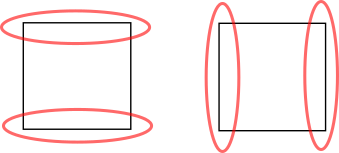
\includegraphics[width=4cm]{order_1_matchings.png}
  	\caption{Matchings on $AD(1)$}
	 \label{fig:ad1}
 	 \end{center}
 \end{minipage}	
 %
 \hspace{1cm}
 \begin{minipage}{.4\textwidth}
 	\begin{center}
 	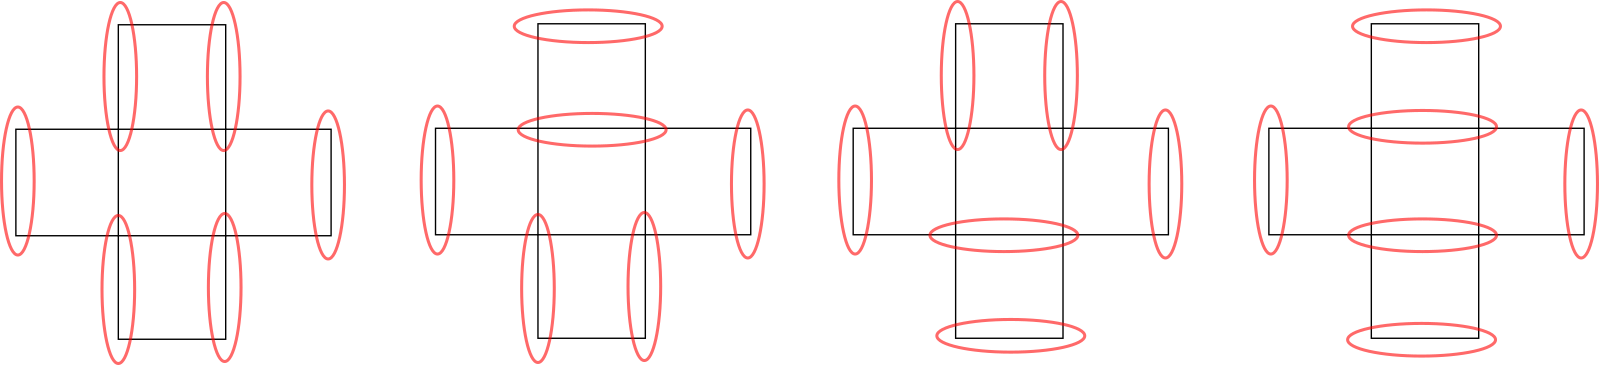
\includegraphics[width=8cm]{order_2_matchings.png}
  	\caption{Matchings on $AD(2)$}
	 \label{fig:ad2}
 	 \end{center}
  \end{minipage}
\end{figure} 
%\end{minipage}	
%%

\hspace{1cm} Note that whenever one of the matchings shown in Figure \ref{fig:ad1} appears within an ambient perfect matching, it can be exchanged with the other in order to produce a new ambient perfect matching. For example, each of the two inner matchings shown in Figure \ref{fig:ad2} is obtained from the other by performing such exchanges on the top and bottom squares. 


\hspace{1cm} We now sketch a proof that the number of perfect matchings on any Aztec Diamond is a power of two. This proof is due to Kuo and Zeilberger and uses the technique of "Graphical Condensation."

\newpage



\subsection*{Claim:} The number of perfect matchings on an Aztec Diamond is a power of two. 

\vspace{1cm}

\subsection*{Sketch of Proof:} 

\hspace{1cm} Our proof will use induction and we have already established the base case. 

To begin the inductive step, consider superimposing two perfect matchings on $AD(n)$. Figure \ref{fig:super} shows one such example in the case that $n = 3$, the ight-most figure showing the matchings laid atop one another. We note that each edge of $AD(3)$ is either in both matchings (a double edge) or falls within a loop defined by the matchings. This example contains four double edges and two loops. It is straightforward to convince oneself that this pattern -- that every edge is either a double edge or in a loop -- is a general phenomenon that occurs whenever two matchings are super imposed. 

\begin{figure}[h]
	\begin{center}
 	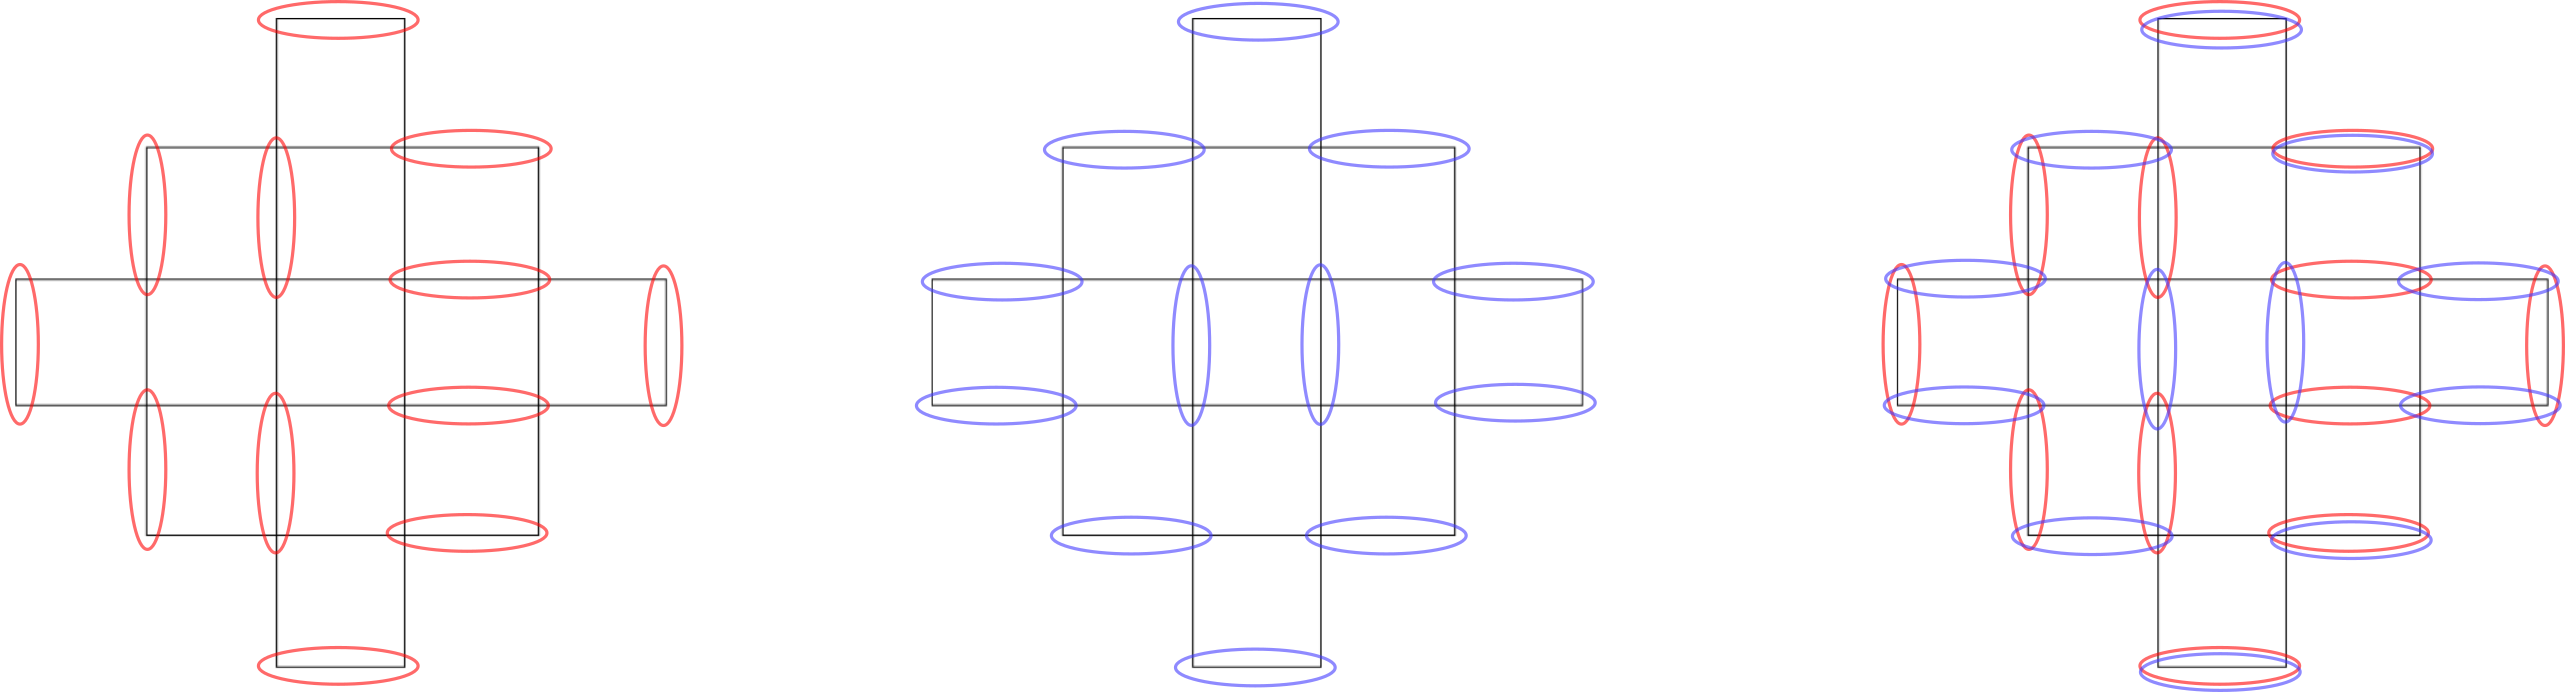
\includegraphics[width=1.2\textwidth]{super_tilings.png}
  	\caption{Matchings of $AD(3)$ Superimposed}
	 \label{fig:super}
 	 \end{center}
\end{figure} 

\hspace{1cm} Now consider what happens when we super-impose a matching on $AD(n-1)$ onto a matching on $AD(n+1)$, with $AD(n-1)$ identified a subgraph of $AD(n+1)$ in the natural way. Figure \ref{fig:super_diag} shows a diagram of the result, with the red representing $AD(n-1)$ and the black showing $AD(n+1)$.  
\begin{figure}[h]
	\begin{center}
 	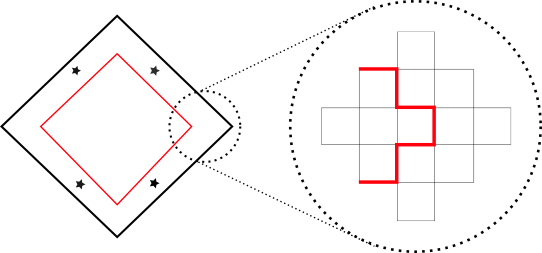
\includegraphics[width=.7\textwidth]{super_diagram.png}
  	\caption{Super Imposed Matchings on $AD(n-1)$ and $AD(n+1)$}
	 \label{fig:super_diag}
 	 \end{center}
\end{figure} 
If $Z(k)$ represents the number of perfect matchings on $AD(k)$ then it is clear that there are $Z(n-1) Z(n+1)$ such diagrams. 

All vertices in $AD(n-1) \cap AD(n+1)$ are used in both perfect matchings. In this sense, we will say that they have degree $2$. On the other hand, those vertices outside of the red square are of degree $1$ as only the perfect matching on $AD(n+1)$ uses them. Note that all vertices in $AD(n-1) \cap AD(n+1)$ are either in a double edge, a loop, or a path defined by the superimposition of the perfect matchings. The first two possibilities occur just as above. If a path occurs, its endpoints must both have degree $1$ and all other vertices must have degree $2$. Thus, a path must start in $AD(n+1) \smallsetminus AD(n-1)$, traverse some part of $AD(n-1)$, and then terminate back in $AD(n+1) \smallsetminus AD(n-1)$. 


Let's focus on the matching near the edges of $AD(n+1)$. Along each of the four edges\footnote{top-left, top-right, bottom-left, bottom-right} the matching resembles that shown in Figure \ref{fig:edge_match}. We notice that for each boundary square the matching must select either the vertical or the horizontal boundary edge and that the only possible ways to do this are: 
\begin{center}
\begin{minipage}{.7\textwidth}
\begin{enumerate}
\item all horizontal edges

\item all vertical edges

\item two sections separated by a distinguished vertex $\star$ where one section consists of horizontal edges and the other consists of vertical edges. 
\end{enumerate}
\end{minipage}
\end{center}
We note that the first two cases are special examples of the third in which one of the two sections is empty. In either case, the vertex $\star$ sits at one of the four corners of the Aztec Diamond. 

\begin{figure}[htb!]
	\begin{center}
 	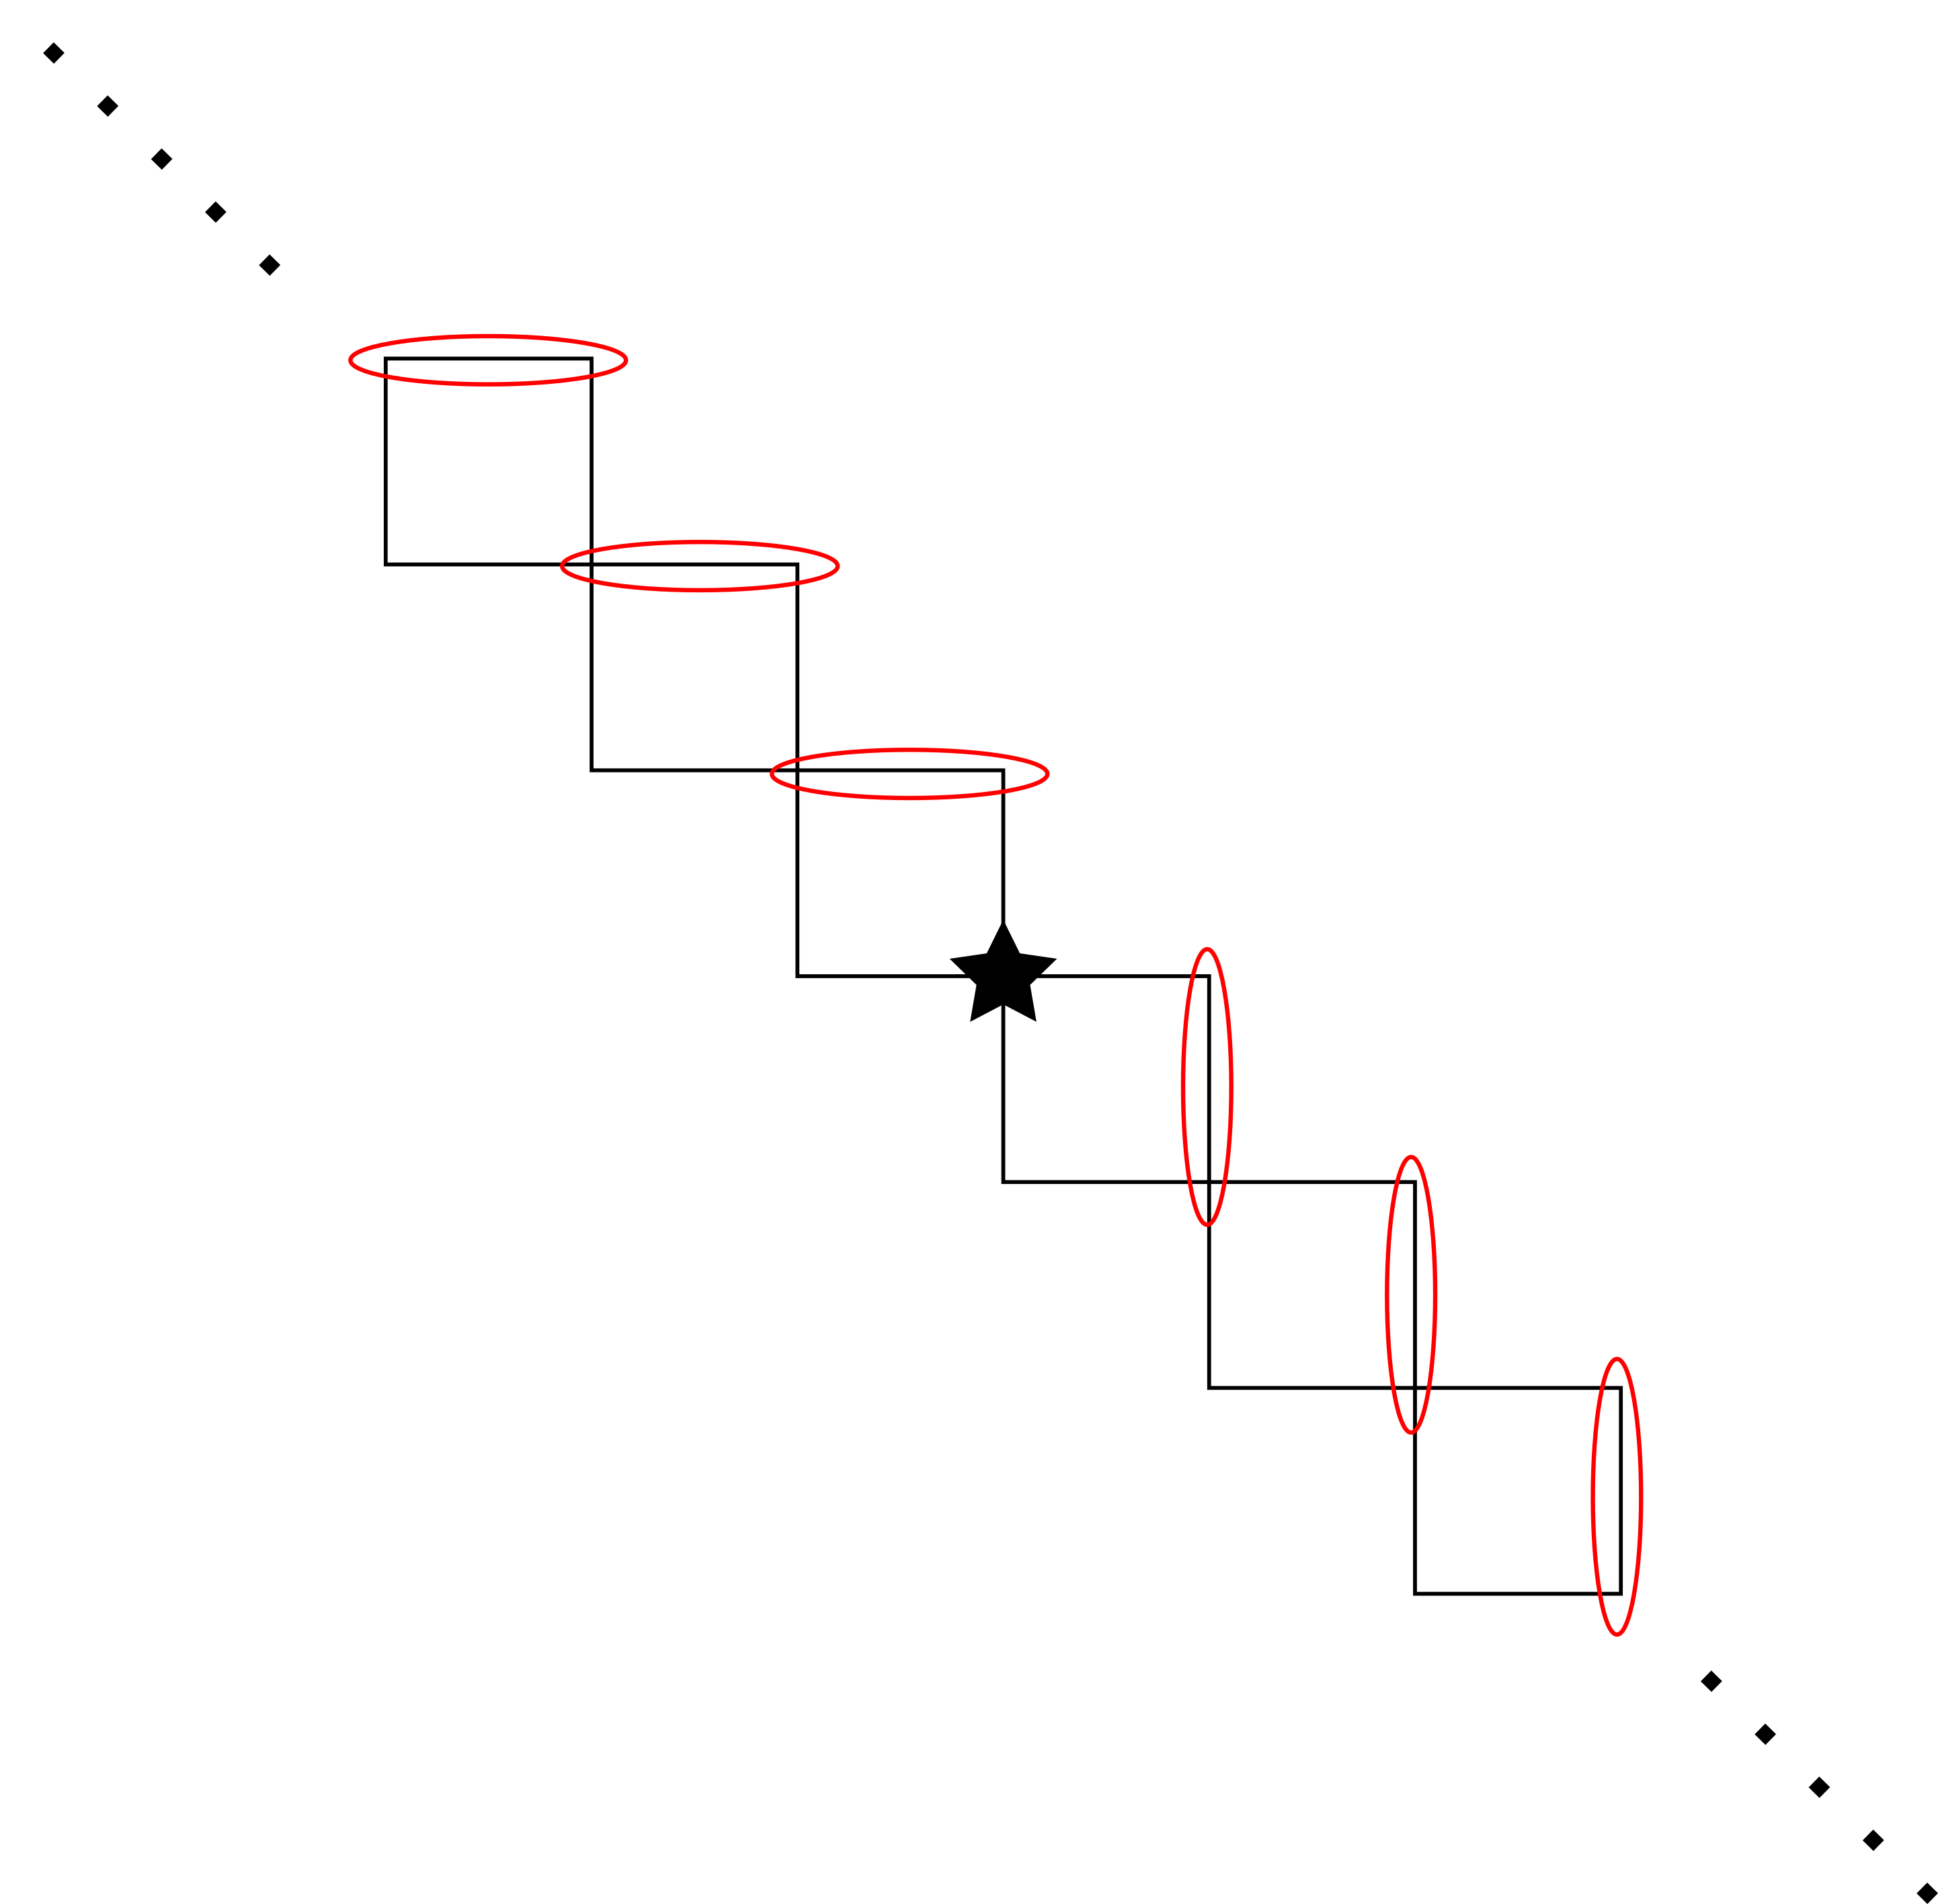
\includegraphics[width=5cm]{edge_match.png}
  	\caption{Matching of $AD(n+1)$ Near Top-Right Edge}
	 \label{fig:edge_match}
 	 \end{center}
\end{figure} 

Observe now that whichever vertex with which $\star$ is paired has degree two as it sits within $AD(n-1)$. Therefore $\star$ must be the endpoint to a path which traverses part of $AD(n-1)$. Each edge of $AD(n+1)$ has exactly one such distinguished vertex\footnote{as shown in the figure} and there therefore must be exactly two disjoint paths through $AD(n-1)$. 


\begin{figure}[htb!]
	\begin{center}
 	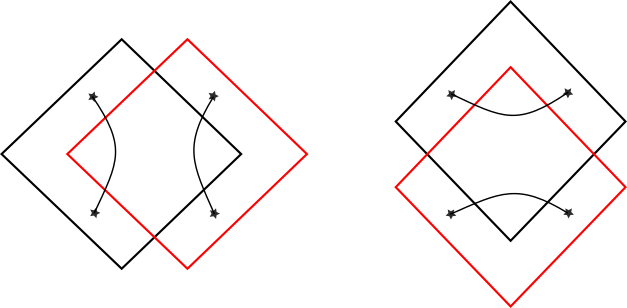
\includegraphics[width=6cm]{offset_match.png}
  	\caption{Offset Matchings of $AD(n)$}
	 \label{fig:offset_match}
 	 \end{center}
\end{figure} 


	We turn now to considering instead what happens when we overlay matchings from two offset copies of $AD(n)$. We can do this either vertically or horizontally, which leads two the two diagrams shown, where the points $\star$ play the same role as before and the paths they determine are shown. Each case determines $Z(n)^2$ possible diagrams so that there are a total of $2Z(n)^2$ possibilities. It can now be shown that these diagrams are in bijection with those obtained from $AD(n+1)$ and $AD(n-1)$.\footnote{this involves rearranging the tiles along the predetermined paths} This gives us the relation 
	$$
	Z(n+1)Z(n-1) = 2 Z(n)^2 \hspace{1cm} \Rightarrow \hspace{1cm} Z(n+1) = \frac{2 Z(n)^2}{Z(n-1)}. 
	$$
Since $Z(1)= 2$ it now follows inductively that $Z(n)$ is a power of two for any $n$. 	$\square$
	
	
	\section{Statistical Mechanics}
	
	\hspace{1cm} We will now begin our work with Statistical Mechanics. In short, Statistical Mechanics works with big systems assembled from simple systems. We then think of the entire system as having many different states determined by the small, local systems, and their interactions. For example, in the Dimer Model, the entire system is the bipartite graph and the different possible states are represented by the different possible perfect matchings. 
	
	For a given system, let $\mathscr{S}$ represent the space of all possible states. We have an energy function $E: \mathscr{S} \rightarrow \mathbb{R}$ that assigns to each state a particular energy. We can then define a probability measure on $\mathscr{S}$ such that  
	$$
	\mathbb{P} \{\text{system is in state } s\} \propto e^{-E(s)/(kT)}
	$$
where $T$ represents the temperature and $k$ is known as "Boltzmann's constant." This type of measure is usually called a "Boltzmann Measure." 

\subsection{Honeycomb Example}

\hspace{1cm} Consider the honeycomb graph shown in Figure \ref{fig:honecomb}. The energy of a perfect matching on this graph is defined to be the product of all edge weights in the matching. Diagonal edges are given weight $1$ and all other weights are labelled in the figure, where $q$ is a constant. 
\begin{figure}[htb!]
	\begin{center}
 	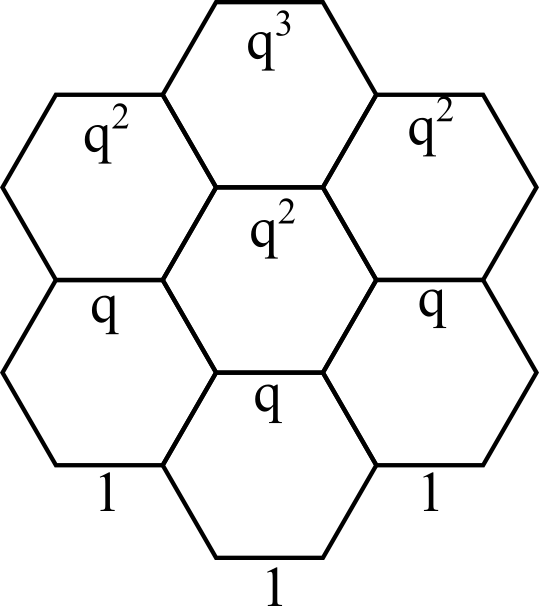
\includegraphics[width=6cm]{honeycomb.png}
  	\caption{Honeycomb Graph}
	 \label{fig:honeycomb}
 	 \end{center}
\end{figure} 
	
	
Let us consider what happens when we change states by altering the perfect matching around one hexagon as shown in Figure \ref{fig:honey_switch}. We see that in the product determining the energy of the matching, a factor of $q^{k}$ is replaced by $q^{k+1}$ so that the total energy increases by a factor of $q$. 
\begin{figure}[htb!]
	\begin{center}
 	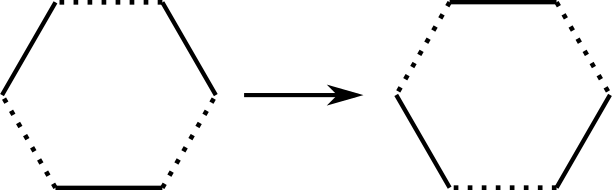
\includegraphics[width=6cm]{honey_switch.png}
  	\caption{Matching Switch}
	 \label{fig:honey_switch}
 	 \end{center}
\end{figure} 
	
The same information is encoded by tiling the plane with rhombuses. The translation is shown in Figure \ref{fig:honey_rhom} 	where we see the edges of each rhombus intersect those edges of the hexagon not in the perfect matching. Moving forward, we will consider the right-hand configuration as a box and the left-hand configuration as the absence of a box. 
\begin{figure}[htb!]
	\begin{center}
 	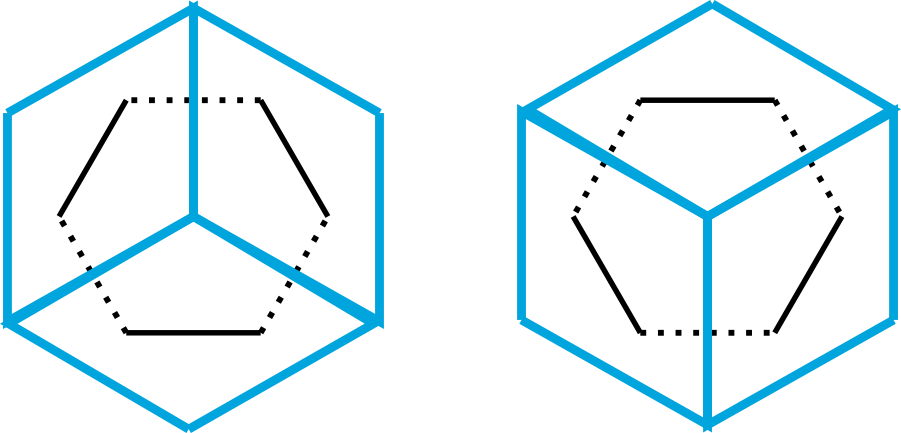
\includegraphics[width=6cm]{honey_rhombus.png}
  	\caption{Matching to Rhombus Plane Partition}
	 \label{fig:honey_rhom}
 	 \end{center}
\end{figure} 

This translates the problem of perfect matchings on the honeycomb graph to one of stacking boxes in the corner of a room. Figure \ref{fig:honey_match_rhom} then shows the beginning of one such stacking configuration, which consists of three boxes. Only the top of one box is visible. 
\begin{figure}[htb!]
	\begin{center}
 	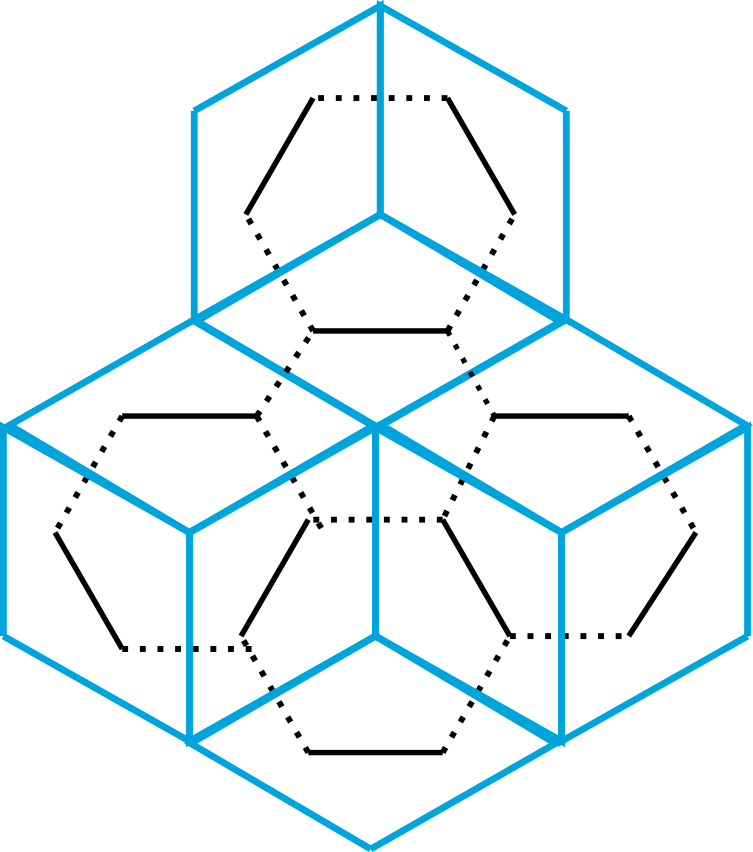
\includegraphics[width=6cm]{honey_match_rhom.png}
  	\caption{Matching as Rhombus Plane Partition}
	 \label{fig:honey_match_rhom}
 	 \end{center}
\end{figure} 

	
	
\end{document}	
